% ថ្នាក់ទី ១១ (វិទ្យាសាស្ត្រ) · ជំពូកទី ១ · មេរៀនទី ៤ · សៀវភៅទំព័រ ២៤–៣៥
\chapter{ផលបូកតួនៃស៊ីតផ្សេងៗ}

\begin{objBox}[វត្ថុបំណង]
\begin{enumerate}[1]
  \item គណនាផលបូកតួនៃស៊ីត
  \item ចេះប្រើនិមិត្តសញ្ញា $\Sigma$ សម្រាប់ផលបូកនៃស៊ីត
  \item កំណត់តួទី $n$ តាមផលសងស៊ីតលំដាប់ $1$ និងលំដាប់ $2$ ។
\end{enumerate}
\end{objBox}

\section{របៀបគណនាផលបូក}

ចំពោះស៊ីតផ្សេងៗ គេពុំអាចប្រើរូបមន្តផលបូកនៃស៊ីតនព្វន្ត ឬស៊ីតធរណីមាត្រមកគណនាផលបូកវាបានឡើយ ក្នុងករណីនេះត្រូវប្រើវិធីផ្សេងៗទៅតាមទម្រង់នៃស៊ីត ។

\begin{example}[ឧទាហរណ៍ ១]
ចំពោះផលបូក $S = 1^2 + 2^2 + 3^2 + \ldots + n^2$ ។

គេអាចគណនាផលបូកនេះដោយប្រើសមភាព $(k+1)^3 - k^3 = 3k^2 + 3k + 1$ ដោយឱ្យ $k$ យកតម្លៃពី $1$ ដល់ $n$
\[
\begin{aligned}
2^3 - 1^3 &= 3 \times 1^2 + 3 \times 1 + 1\\
3^3 - 2^3 &= 3 \times 2^2 + 3 \times 2 + 1\\
4^3 - 3^3 &= 3 \times 3^2 + 3 \times 3 + 1\\
&\ \,\vdots\\
n^3 - (n-1)^3 &= 3 \times (n-1)^2 + 3 \times (n-1) + 1 &\quad (1)\\
(n+1)^3 - n^3 &= 3 \times n^2 + 3 \times n + 1 &\quad (2)
\end{aligned}
\]
បូកអង្គនិងអង្គនៃសមីការ $(1)$ និង $(2)$ គេបាន
\[
\begin{aligned}
(n+1)^3 - 1^3 &= 3 \times (1^2 + 2^2 + 3^2 + \ldots + n^2)\\
&\quad + 3 \times (1 + 2 + 3 + \ldots + n)\\
&\quad + (1 + 1 + 1 + \ldots + 1)\\
&= 3 \times S + 3 \times \frac{n(n+1)}{2} + n \text{ ។}
\end{aligned}
\]
គណនា $S$ គេបាន $1^2 + 2^2 + 3^2 + \ldots + n^2 = \dfrac{n(n+1)(2n+1)}{6}$ ។
\end{example}

\begin{example}[ឧទាហរណ៍ ២]
ចំពោះផលបូក $S = \dfrac{1}{1 \cdot 2} + \dfrac{1}{2 \cdot 3} + \dfrac{1}{3 \cdot 4} + \ldots + \dfrac{1}{n \cdot (n+1)}$ ។

គេអាចគណនាផលបូកនេះដោយប្រើសមភាព $\dfrac{1}{k \cdot (k+1)} = \dfrac{1}{k} - \dfrac{1}{k+1}$ ដោយឱ្យ $k$ យកតម្លៃពី $1$ ដល់ $n$
\[
\begin{aligned}
\frac{1}{1 \cdot 2} &= \frac{1}{1} - \frac{1}{2}\\
\frac{1}{2 \cdot 3} &= \frac{1}{2} - \frac{1}{3}\\
\frac{1}{3 \cdot 4} &= \frac{1}{3} - \frac{1}{4}\\
&\ \,\vdots\\
\frac{1}{(n-1) \cdot n} &= \frac{1}{n-1} - \frac{1}{n}\\
\frac{1}{n \cdot (n+1)} &= \frac{1}{n} - \frac{1}{n+1}
\end{aligned}
\]
បូកអង្គនិងអង្គនៃសមីការ គេបាន $S = 1 - \dfrac{1}{n+1}$ ។

ដូច្នេះ $\dfrac{1}{1 \cdot 2} + \dfrac{1}{2 \cdot 3} + \dfrac{1}{3 \cdot 4} + \ldots + \dfrac{1}{n \cdot (n+1)} = 1 - \dfrac{1}{n+1} = \dfrac{n}{n+1}$ ។
\end{example}

\begin{example}[លំហាត់គំរូ]
គណនាផលបូក $S = 1^3 + 2^3 + 3^3 + \ldots + n^3$ ។
\end{example}
\ans
គេអាចគណនាផលបូកនេះដោយប្រើសមភាព $(k+1)^4 - k^4 = 4k^3 + 6k^2 + 4k + 1$ ដោយឱ្យ $k$ យកតម្លៃពី $1$ ដល់ $n$
\[
\begin{aligned}
2^4 - 1^4 &= 4 \times 1^3 + 6 \times 1^2 + 4 \times 1 + 1\\
3^4 - 2^4 &= 4 \times 2^3 + 6 \times 2^2 + 4 \times 2 + 1\\
4^4 - 3^4 &= 4 \times 3^3 + 6 \times 3^2 + 4 \times 3 + 1\\
&\ \,\vdots\\
n^4 - (n-1)^4 &= 4 \times (n-1)^3 + 6 \times (n-1)^2\\
&\quad + 4 \times (n-1) + 1\\
(n+1)^4 - n^4 &= 4 \times n^3 + 6 \times n^2 + 4 \times n + 1
\end{aligned}
\]
បូកអង្គនិងអង្គនៃសមីការ គេបាន
\[
\begin{aligned}
(n+1)^4 - 1^4 &= 4 \times (1^3 + 2^3 + 3^3 + \ldots + n^3)\\
&\quad + 6 \times (1^2 + 2^2 + 3^2 + \ldots + n^2)\\
&\quad + 4 \times (1 + 2 + 3 + \ldots + n) + (1 + 1 + 1 + \ldots + 1)\\
&= 4S\\
&\quad + 6 \times (1^2 + 2^2 + 3^2 + \ldots + n^2)\\
&\quad + 4 \times (1 + 2 + 3 + \ldots + n)\\
&\quad + (1 + 1 + 1 + \ldots + 1)
\end{aligned}
\]
គណនា $S$ គេបាន $1^3 + 2^3 + 3^3 + \ldots + n^3 = \dfrac{n^2(n+1)^2}{4} = \left[\dfrac{n(n+1)}{2}\right]^2$ ។

\begin{pro}
\begin{enumerate}[1]
  \item គណនា $S = 12^3 + 13^3 + 14^3 + \ldots + 50^3$ ។
  \item គណនា $S = \dfrac{1}{1 \cdot 2 \cdot 3} + \dfrac{1}{2 \cdot 3 \cdot 4} + \dfrac{1}{3 \cdot 4 \cdot 5} + \ldots + \dfrac{1}{n \cdot (n+1) \cdot (n+2)}$ ។
\end{enumerate}
\ans
\begin{enumerate}[1]
  \item $S = 1621269$
  \item $S = \dfrac{1}{2}\left(\dfrac{1}{2} - \dfrac{1}{(n+1)(n+2)}\right)$ ។
\end{enumerate}
\end{pro}

\section{គណនាផលបូកតាមលំនាំគំរូ}

ចំពោះស៊ីតដែលមានតួជាចំនួនគត់ គេអាចគណនាផលបូកវាតាមការសង្កេតលំនាំគំរូ ។

\begin{example}[ឧទាហរណ៍]
\[
\begin{aligned}
1 &= 1 = 1^2\\
1 + 3 &= 4 = 2^2\\
1 + 3 + 5 &= 9 = 3^2\\
1 + 3 + 5 + 7 &= 16 = 4^2
\end{aligned}
\]
\begin{center}
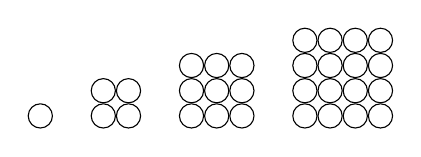
\begin{tikzpicture}[scale=0.32]
  \foreach \n/\x in {1/0, 2/2.5, 3/6, 4/10.5}
    \foreach \i in {1,...,\n} \foreach \j in {1,...,\n}
      \draw (\x+\i,\j) circle (0.48);
\end{tikzpicture}
\end{center}
ដូច្នេះ $1 + 3 + 5 + \ldots + (2n - 1) = n^2$ ។
\end{example}

\begin{example}[លំហាត់គំរូ]
គណនាផលបូក $n$ តួនៃចំនួនគូ $S = 2 + 4 + 6 + \ldots + 2n$ ។
\end{example}
\ans
\[
\begin{aligned}
2 &= 2 = 1 \times 2\\
2 + 4 &= 6 = 2 \times 3\\
2 + 4 + 6 &= 12 = 3 \times 4\\
2 + 4 + 6 + 8 &= 20 = 4 \times 5
\end{aligned}
\]
\begin{center}
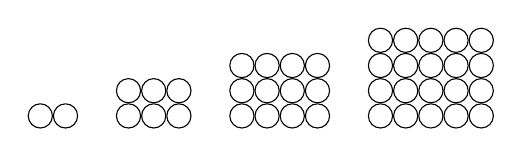
\begin{tikzpicture}[scale=0.32]
  \foreach \n/\x in {1/0, 2/3.5, 3/8, 4/13.5}
    \foreach \i in {1,...,\n} \foreach \j in {1,...,\the\numexpr\n+1\relax}
      \draw (\x+\j,\i) circle (0.48);
\end{tikzpicture}
\end{center}
ដូច្នេះ $2 + 4 + 6 + \ldots + 2n = n \cdot (n + 1)$ ។

\begin{pro}
គេឱ្យលំនាំគំរូនៃស៊ីតខាងក្រោម ៖
\[
\begin{aligned}
1 &= 1\\
1 + 7 &= 8\\
1 + 7 + 19 &= 27\\
1 + 7 + 19 + 37 &= 64\\
1 + 7 + 19 + 37 + 61 &= 125
\end{aligned}
\]
គណនាផលបូកនៃស៊ីតនេះដែលមាន $10$ តួ ។
\ans
$S = 1000$ ។
\end{pro}

\section{និមិត្តសញ្ញា \texorpdfstring{$\Sigma$}{Σ} សម្រាប់ផលបូកនៃស៊ីត}
\subsection{សញ្ញាណ \texorpdfstring{$\Sigma$}{Σ}}

ក្នុងការសរសេរផលបូកតួនៃស៊ីត $a_1, a_2, a_3, \ldots, a_n$ គេប្រើនិមិត្តសញ្ញា $\Sigma$ អានថា \textbf{ស៊ិចម៉ា} សម្រាប់តាងផលបូក $n$ តួនៃស៊ីត ។ គេកំណត់សរសេរ
\[ \sum_{k=1}^{n} a_k = a_1 + a_2 + a_3 + \ldots + a_n \text{ ។} \]
ក្នុងនោះ $k$ យកតម្លៃពី $1, 2, 3, \ldots$ រហូតដល់ $n$ ។

\begin{example}[ឧទាហរណ៍]
\[
\begin{gathered}
1 + 2 + 3 + \ldots + n = \sum_{k=1}^{n} k = \frac{n(n+1)}{2} \text{ ។}\\
\begin{aligned}
1^2 + 2^2 + 3^2 + \ldots + n^2 &= \sum_{k=1}^{n} k^2\\
&= \frac{n(n+1)(2n+1)}{6} \text{ ។}
\end{aligned}
\end{gathered}
\]
\end{example}

\begin{example}[លំហាត់គំរូ ១]
សរសេរផលបូកខាងក្រោមដោយប្រើនិមិត្តសញ្ញា $\Sigma$ ៖
\begin{enumerate}[a]
  \item $1^3 + 2^3 + 3^3 + \ldots + n^3$
  \item $2 + 4 + 6 + 8 + \ldots + 100$
  \item $\frac{1}{2} - \frac{1}{3} + \frac{1}{4} - \frac{1}{5} + \ldots + \frac{1}{50}$ ។
\end{enumerate}
\end{example}
\ans
\begin{enumerate}[a]
  \item $1^3 + 2^3 + 3^3 + \ldots + n^3 = \displaystyle\sum_{k=1}^{n} k^3 = \left[\frac{n(n+1)}{2}\right]^2$ ។
  \item $2 + 4 + 6 + 8 + \ldots + 100 = 2 \times 1 + 2 \times 2 + 2 \times 3 + \ldots + 2 \times 50$\\
  ផលបូកស៊ីតនេះមានតួទូទៅ $2n$ ហើយ $n$ យកតម្លៃពី $1$ ដល់ $50$ ។ គេបាន $2 + 4 + 6 + 8 + \ldots + 100 = \displaystyle\sum_{n=1}^{50} 2n$ ។
  \item $\frac{1}{2} - \frac{1}{3} + \frac{1}{4} - \frac{1}{5} + \ldots + \frac{1}{50}$ ផលបូកស៊ីតនេះមានតួទូទៅនៃស៊ីត $\dfrac{(-1)^n}{n}$ ចំពោះ $n$ យកតម្លៃពី $2$ ដល់ $50$ ។\\
  គេបាន $\dfrac{1}{2} - \dfrac{1}{3} + \dfrac{1}{4} - \dfrac{1}{5} + \ldots + \dfrac{1}{50} = \displaystyle\sum_{n=2}^{50} \frac{(-1)^n}{n}$ ។
\end{enumerate}

\begin{example}[លំហាត់គំរូ ២]
សរសេរគ្រប់តួទាំងអស់នៃផលបូកដោយមិនប្រើនិមិត្តសញ្ញា $\Sigma$
\begin{tasks}(3)
  \task $\displaystyle\sum_{k=1}^{6} 2$
  \task $\displaystyle\sum_{n=2}^{5} (2n + 1)$
  \task $\displaystyle\sum_{j=1}^{5} j(j+1)$ ។
\end{tasks}
\end{example}
\ans
\begin{enumerate}[a]
  \item $\displaystyle\sum_{k=1}^{6} 2 = 2 + 2 + 2 + 2 + 2 + 2$ ។
  \item $\displaystyle\sum_{n=2}^{5} (2n + 1) = 5 + 7 + 9 + 11$ ។
  \item $\displaystyle\sum_{j=1}^{5} j(j+1) = 2 + 6 + 12 + 20 + 30$ ។
\end{enumerate}

\begin{pro}
សរសេរផលបូកខាងក្រោមដោយប្រើនិមិត្តសញ្ញា $\Sigma$ ៖
\begin{enumerate}[a]
  \item $2 + 5 + 8 + \ldots + (3n - 1)$
  \item $3 + 6 + 12 + \ldots + 3(2)^{n-1}$
  \item $1 + \frac{1}{2} + \frac{1}{3} + \frac{1}{4} + \ldots + \frac{1}{100}$ ។
\end{enumerate}
\ans
\begin{tasks}(3)
  \task $\displaystyle\sum_{k=1}^{n} (3k - 1)$
  \task $\displaystyle\sum_{k=1}^{n} 3 \times 2^{k-1}$
  \task $\displaystyle\sum_{k=1}^{100} \frac{1}{k}$ ។
\end{tasks}
\end{pro}

\subsection{លក្ខណៈនៃស៊ិចម៉ា}

\begin{formulaBox}[លក្ខណៈ]
\begin{enumerate}[a]
  \item $\displaystyle\sum_{k=1}^{n} c = nc$
  \item $\displaystyle\sum_{k=1}^{n} c a_k = c \sum_{k=1}^{n} a_k$
  \item $\displaystyle\sum_{k=1}^{n} (a_k + b_k) = \sum_{k=1}^{n} a_k + \sum_{k=1}^{n} b_k$
  \item $\displaystyle\sum_{k=1}^{n} (a_k - b_k) = \sum_{k=1}^{n} a_k - \sum_{k=1}^{n} b_k$
  \item $\displaystyle\sum_{k=1}^{n} (a_k + b_k)^2 = \sum_{k=1}^{n} a_k^2 + 2\sum_{k=1}^{n} a_k b_k + \sum_{k=1}^{n} b_k^2$ ។
\end{enumerate}
\end{formulaBox}

\textbf{សម្រាយបញ្ជាក់}
\begin{enumerate}[a]
  \item $\displaystyle\sum_{k=1}^{n} c = c + c + c + \ldots + c = nc$ ។
  \item $\displaystyle\sum_{k=1}^{n} c a_k = c a_1 + c a_2 + c a_3 + \ldots + c a_n = c(a_1 + a_2 + a_3 + \ldots + a_n) = c \sum_{k=1}^{n} a_k$ ។
  \item $\displaystyle\sum_{k=1}^{n} (a_k + b_k) = (a_1 + b_1) + (a_2 + b_2) + \ldots + (a_n + b_n) = (a_1 + a_2 + \ldots + a_n) + (b_1 + b_2 + \ldots + b_n) = \sum_{k=1}^{n} a_k + \sum_{k=1}^{n} b_k$ ។
  \item $\displaystyle\sum_{k=1}^{n} (a_k - b_k) = (a_1 - b_1) + (a_2 - b_2) + \ldots + (a_n - b_n) = (a_1 + a_2 + \ldots + a_n) - (b_1 + b_2 + \ldots + b_n) = \sum_{k=1}^{n} a_k - \sum_{k=1}^{n} b_k$ ។
  \item $\displaystyle\sum_{k=1}^{n} (a_k + b_k)^2 = \sum_{k=1}^{n} (a_k^2 + 2a_k b_k + b_k^2) = \sum_{k=1}^{n} a_k^2 + 2\sum_{k=1}^{n} a_k b_k + \sum_{k=1}^{n} b_k^2$ ។
\end{enumerate}

\begin{example}[លំហាត់គំរូ]
គណនា \quad ក. $\displaystyle\sum_{k=1}^{15} (4k + 3)$ \quad ខ. $\displaystyle\sum_{k=1}^{20} (k + 3)k$ ។
\end{example}
\ans
\begin{enumerate}[a]
  \item \[
  \begin{aligned}
\sum_{k=1}^{15} (4k + 3) &= \sum_{k=1}^{15} 4k\\
&\quad + \sum_{k=1}^{15} 3\\
&= 4\sum_{k=1}^{15} k\\
&\quad + \sum_{k=1}^{15} 3\\
&= 4(1 + 2 + 3 + \ldots + 15)\\
&\quad + 15 \times 3\\
&= 4 \times \frac{(1 + 15) \times 15}{2} + 45\\
&= 2 \times 16 \times 15 + 45 = 525 \text{ ។}
\end{aligned}
  \]
  \item \[
  \begin{aligned}
\sum_{k=1}^{20} (k + 3)k &= \sum_{k=1}^{20} (k^2 + 3k)\\
&= \sum_{k=1}^{20} k^2\\
&\quad + 3\sum_{k=1}^{20} k\\
&= \frac{20 \times 21 \times 41}{6} + 3\,\frac{21 \times 20}{2}\\
&= 10 \times 7 \times 41 + 3 \times 21 \times 10\\
&= 2870 + 630 = 3500 \text{ ។}
\end{aligned}
  \]
\end{enumerate}

\begin{pro}
គណនា
\begin{tasks}(3)
  \task $\displaystyle\sum_{k=1}^{20} (3k + 1)$
  \task $\displaystyle\sum_{k=1}^{7} 2^k$
  \task $\displaystyle\sum_{k=4}^{14} (4k - 3)$
  \task $\displaystyle\sum_{k=1}^{n} (3 + k)^2$
  \task $\displaystyle\sum_{k=1}^{30} k(k+1)$ ។
\end{tasks}
\ans
\begin{tasks}(3)
  \task $\displaystyle\sum_{k=1}^{20} (3k + 1) = 650$
  \task $\displaystyle\sum_{k=1}^{7} 2^k = 254$
  \task $\displaystyle\sum_{k=4}^{14} (4k - 3) = 363$
  \task $\displaystyle\sum_{k=1}^{n} (3 + k)^2 = \frac{n}{6}(2n^2 + 21n + 73)$
  \task $\displaystyle\sum_{k=1}^{30} k(k+1) = 9920$ ។
\end{tasks}
\end{pro}

\section{របៀបកំណត់តួទី \texorpdfstring{$n$}{n} តាមផលសងតួនៃស៊ីត}

គេអាចកំណត់តួទី $n$ របស់ស៊ីត $(a_n)$ ដែលពុំមែនជាស៊ីតនព្វន្ត ឬជាស៊ីតធរណីមាត្រតាមរបៀបដូចខាងក្រោម ៖

\subsection{ផលសងតួលំដាប់ទី ១ នៃស៊ីត}

\begin{example}[ឧទាហរណ៍ ១]
កំណត់តួទី $n$ នៃស៊ីត $1, 3, 7, 13, 21, 31, \ldots$ ។

គេសង្កេតឃើញថាស៊ីតនេះមិនមែនជាស៊ីតនព្វន្ត ហើយក៏មិនមែនជាស៊ីតធរណីមាត្រ ។ នោះគេត្រូវធ្វើផលសងនៃតួបន្តបន្ទាប់គ្នានៃស៊ីត $1, 3, 7, 13, 21, 31, \ldots$ ។ គេបានលំនាំគំរូដូចជា
\begin{center}
\begin{tabular}{lcccccc}
$n$ & $1$ & $2$ & $3$ & $4$ & $5$ & $6\ldots$\\
ស៊ីត $(a_n)$ & $1$ & $3$ & $7$ & $13$ & $21$ & $31\ldots$\\
ផលសងតួលំដាប់ទី ១ នៃស៊ីត & $2$ & $4$ & $6$ & $8$ & $10\ldots$ &
\end{tabular}
\end{center}
ផលសងតួនៃស៊ីតអាចជួយឱ្យគេរកលំនាំគំរូ ដែលអាចកំណត់តួទូទៅនៃស៊ីតបានដូចជា
\[
\begin{aligned}
a_2 - a_1 &= 3 - 1 = 2 \times 1\\
a_3 - a_2 &= 7 - 3 = 4 = 2 \times 2\\
a_4 - a_3 &= 13 - 7 = 6 = 2 \times 3\\
&\ \,\vdots\\
a_{n-1} - a_{n-2} &= 2 \times (n - 2)\\
a_n - a_{n-1} &= 2 \times (n - 1)
\end{aligned}
\]
បូកអង្គនិងអង្គទាំងអស់ គេបាន
\[
\begin{aligned}
a_n - a_1 = a_n - 1 &= 2 \times 1 + 2 \times 2 + 2 \times 3 + \ldots\\
&\quad + 2 \times (n - 2) + 2 \times (n - 1)\\
a_n &= 2 \times 1 + 2 \times 2 + 2 \times 3 + \ldots\\
&\quad + 2 \times (n - 2) + 2 \times (n - 1)\\
&\quad + 1\\
&= 2 \times [1 + 2 + 3 + \ldots + (n - 2) + (n - 1)]\\
&\quad + 1\\
&= 2 \times \frac{[1 + (n - 1)](n - 1)}{2}\\
&\quad + 1\\
&= n(n - 1) + 1 = n^2 - n + 1
\end{aligned}
\]
ដូច្នេះតួទី $n$ នៃស៊ីត $1, 3, 7, 13, 21, 31, \ldots$ កំណត់ដោយ $a_n = n^2 - n + 1$ ។
\end{example}

\begin{formulaBox}[ជាទូទៅ]
គេមានស៊ីត $(a_n)$ ៖ $a_1, a_2, a_3, \ldots, a_n$ ហើយ $b_1 = a_2 - a_1$, $b_2 = a_3 - a_2$, $b_3 = a_4 - a_3$, $\ldots$, $b_{n-1} = a_n - a_{n-1}$ ។

ស៊ីត $(b_n)$ ៖ $b_1, b_2, b_3, \ldots, b_{n-1}$ ហៅថាផលសងតួលំដាប់ទី $1$ នៃស៊ីត $(a_n)$ ។
\end{formulaBox}

\begin{example}[ឧទាហរណ៍ ២]
បង្ហាញថា $a_n = a_1 + \displaystyle\sum_{k=1}^{n-1} b_k$ ចំពោះ $n \ge 2$ ។
\[
\begin{cases}
a_2 - a_1 = b_1\\
a_3 - a_2 = b_2\\
a_4 - a_3 = b_3\\
\quad\vdots\\
a_{n-1} - a_{n-2} = b_{n-2}\\
a_n - a_{n-1} = b_{n-1}
\end{cases}
\]
បូកអង្គនិងអង្គ គេបាន $a_n - a_1 = b_1 + b_2 + b_3 + \ldots + b_{n-1}$ ។

ចំពោះ $n \ge 2$ គេបាន $a_n = a_1 + (b_1 + b_2 + b_3 + \ldots + b_{n-1}) = a_1 + \displaystyle\sum_{k=1}^{n-1} b_k$ ។

ចំពោះ $n = 1$ គេបាន $b_{n-1} = b_0$ មិនមាន ។ ដូច្នេះ $a_n = a_1 + \displaystyle\sum_{k=1}^{n-1} b_k$ ចំពោះ $n \ge 2$ ។
\end{example}

\begin{formulaBox}[ជាទូទៅ]
គេមានស៊ីត $(a_n)$ និងស៊ីត $(b_n)$ ដែលកំណត់ដោយ $b_n = a_{n+1} - a_n$, $n = 1, 2, 3, \ldots$ តួទី $n$ នៃស៊ីត $(a_n)$ កំណត់ដោយ $a_n = a_1 + \displaystyle\sum_{k=1}^{n-1} b_k$ ចំពោះ $n \ge 2$ ។
\end{formulaBox}

\begin{example}[លំហាត់គំរូ ១]
កំណត់តួទី $n$ នៃស៊ីត $2, 4, 8, 14, 22, 32, \ldots$ ។
\end{example}
\ans
តាង $a_n$ ជាតួទី $n$ នៃស៊ីតដែលគេឱ្យ ។ ស៊ីត $(b_n)$ ជាផលសងតួលំដាប់ទី $1$ នៃស៊ីត $(a_n)$ ដែលមានតួ $b_n$ កំណត់ដោយ $b_n = a_{n+1} - a_n$ ។

ស៊ីត $(b_n)$ ៖ $2, 4, 6, 8, \ldots$ ។ ស៊ីត $(b_n)$ ជាស៊ីតនព្វន្តដែលមានតួទី $1$ ស្មើនឹង $2$ និងផលសងរួមស្មើនឹង $2$ នោះ $b_n = 2 + 2(n - 1) = 2n$ ។

ចំពោះ $n \ge 2$ គេបាន
\[
\begin{aligned}
a_n &= a_1 + \sum_{k=1}^{n-1} b_k = 2 + \sum_{k=1}^{n-1} 2k\\
&= 2 + 2 \cdot \frac{1}{2}n(n - 1) = 2 + n^2 - n = n^2 - n + 2
\end{aligned}
\]
នោះ $a_n = n^2 - n + 2$ ។ ចំពោះ $n = 1$, $a_1 = 1^2 - 1 + 2 = 2$ ពិត ។

ដូច្នេះស៊ីត $(a_n)$ មានតួទី $n$ កំណត់ដោយ $a_n = n^2 - n + 2$ ។

\begin{example}[លំហាត់គំរូ ២]
\begin{enumerate}[a]
  \item កំណត់តួទី $n$ នៃស៊ីត $1, 2, 5, 10, 17, \ldots$ ។
  \item គណនាផលបូក $n$ តួដំបូងនៃស៊ីតនេះ ។
\end{enumerate}
\end{example}
\ans
\begin{enumerate}[a]
  \item កំណត់តួទី $n$ នៃស៊ីត $(a_n)$ ៖ $1, 2, 5, 10, 17, \ldots$ ។ តាង $a_n$ ជាតួទី $n$ នៃស៊ីតដែលគេឱ្យ $(a_n)$ ។ ស៊ីត $(b_n)$ ជាផលសងតួលំដាប់ទី $1$ នៃស៊ីត $(a_n)$ ដែលមានតួ $b_n$ កំណត់ដោយ $b_n = a_{n+1} - a_n$ ។

  ស៊ីត $(b_n)$ ៖ $1, 3, 5, 7, \ldots$ ។ ស៊ីត $(b_n)$ ជាស៊ីតនព្វន្តដែលមានតួទី $1$ ស្មើនឹង $1$ និងផលសងរួមស្មើនឹង $2$ នោះ $b_n = 1 + 2(n - 1) = 2n - 1$ ។

  ចំពោះ $n \ge 2$ គេបាន
  \[
  \begin{aligned}
a_n &= a_1 + \sum_{k=1}^{n-1} b_k\\
&= 1 + \sum_{k=1}^{n-1} (2k - 1)\\
&= 1 + 2\sum_{k=1}^{n-1} k - (n - 1)\\
&= 1 + 2 \cdot \frac{1}{2}n(n - 1) - (n - 1)\\
&= 1 + n^2 - n - n + 1 = 2 - 2n + n^2
\end{aligned}
  \]
  នោះ $a_n = 2 - 2n + n^2$ ។ ចំពោះ $n = 1$ គេបាន $a_1 = 2 - 2 + 1 = 1$ ពិត ។ ដូច្នេះ $a_n = 2 - 2n + n^2$ ។
  \item គណនាផលបូក $n$ តួដំបូងនៃស៊ីត $(a_n)$ ។ តាង $S_n$ ជាផលបូកនៃស៊ីត $(a_n)$ គឺ
  \[
  \begin{aligned}
S_n &= a_1 + a_2 + a_3 + \ldots + a_n = \sum_{k=1}^{n} (2 - 2k + k^2)\\
&= 2n - 2\sum_{k=1}^{n} k + \sum_{k=1}^{n} k^2\\
&= 2n - 2 \cdot \frac{1}{2}n(n + 1)\\
&\quad + \frac{1}{6}n(n + 1)(2n + 1)\\
&= \frac{12n}{6} - \frac{6}{6}n(n + 1)\\
&\quad + \frac{1}{6}n(n + 1)(2n + 1)\\
&= \frac{1}{6}n(12 - 6n - 6 + 2n^2 + n + 2n + 1)\\
&= \frac{1}{6}n(7 - 3n + 2n^2)
\end{aligned}
  \]
  ដូច្នេះ $S_n = \dfrac{1}{6}n(2n^2 - 3n + 7)$ ។
\end{enumerate}

\begin{pro}
\begin{enumerate}[1]
  \item ក. កំណត់តួទី $n$ នៃស៊ីត $4, 5, 7, 10, 14, \ldots$ ។\\
  ខ. គណនាផលបូក $n$ តួដំបូងនៃស៊ីតនេះ ។
  \item ក. កំណត់តួទី $n$ នៃស៊ីត $3, 5, 8, 12, 17, 23, \ldots$ ។\\
  ខ. គណនាផលបូក $n$ តួដំបូងនៃស៊ីតនេះ ។
\end{enumerate}
\ans
\begin{enumerate}[1]
  \item ក. $a_n = 4 - \dfrac{n}{2} + \dfrac{n^2}{2}$ \quad ខ. $S_n = \dfrac{n(23 + n^2)}{6}$ ។
  \item ក. $a_n = 3 + \dfrac{(n - 1)(n + 2)}{2}$ \quad ខ. $S_n = \dfrac{n}{6}(n^2 + 3n + 14)$ ។
\end{enumerate}
\end{pro}

\subsection{ផលសងតួលំដាប់ទី ២ នៃស៊ីត}

បើសិនជាស៊ីត $(b_n)$ នៅតែមិនអាចកំណត់តួទី $n$ នៃស៊ីត $(a_n)$ បានទៀត នោះគេត្រូវធ្វើផលសងលំដាប់តួនៃស៊ីត $(b_n)$ បន្តទៀត ដែលគេហៅថា ផលសងតួលំដាប់ទី $2$ នៃស៊ីត $(a_n)$ ។

\begin{example}[ឧទាហរណ៍]
កំណត់តួទី $n$ នៃស៊ីត $(a_n)$ ៖ $1, 2, 6, 15, 31, 56, \ldots$ ។

\textbf{របៀបទី ១}
\begin{center}
\begin{tabular}{lcccccc}
$n$ & $1$ & $2$ & $3$ & $4$ & $5$ & $6\ldots$\\
ស៊ីត $(a_n)$ & $1$ & $2$ & $6$ & $15$ & $31$ & $56\ldots$\\
ផលសងតួលំដាប់ទី ១ & $1$ & $4$ & $9$ & $16$ & $25\ldots$ &
\end{tabular}
\end{center}
តាង $a_n$ ជាតួទី $n$ នៃស៊ីត $(a_n)$ ។ ស៊ីត $(b_n)$ ជាផលសងតួលំដាប់ទី $1$ នៃស៊ីត $(a_n)$ ៖ $1, 4, 9, 16, 25, \ldots$ នោះ $b_n = n^2$ ។

ចំពោះ $n \ge 2$ គេបាន $a_n = a_1 + \displaystyle\sum_{k=1}^{n-1} k^2 = 1 + \frac{1}{6}(2n - 1)(n - 1)n$ នោះ $a_n = \dfrac{1}{6}(2n - 1)(n - 1)n + 1$ ។

ចំពោះ $n = 1$, $a_1 = 1$ ពិត ។ ដូច្នេះ $a_n = \dfrac{1}{6}(2n - 1)(n - 1)n + 1$ ។

\textbf{របៀបទី ២}
\begin{center}
\begin{tabular}{lcccccc}
$n$ & $1$ & $2$ & $3$ & $4$ & $5$ & $6\ldots$\\
ស៊ីត $(a_n)$ & $1$ & $2$ & $6$ & $15$ & $31$ & $56\ldots$\\
ផលសងតួលំដាប់ទី ១ & $1$ & $4$ & $9$ & $16$ & $25\ldots$ &\\
ផលសងតួលំដាប់ទី ២ & $3$ & $5$ & $7$ & $9\ldots$ & &
\end{tabular}
\end{center}
តាង $a_n$ ជាតួទី $n$ នៃស៊ីត $(a_n)$ ។ ស៊ីត $(b_n)$ ជាផលសងតួលំដាប់ទី $1$ នៃស៊ីត $(a_n)$ ដែលមានតួទី $n$ នៃស៊ីតគឺ $b_n = a_{n+1} - a_n$ ។

តាង $c_n$ ជាផលសងតួនៃស៊ីត $(b_n)$ ហៅថា ផលសងតួលំដាប់ទី $2$ នៃស៊ីត $(a_n)$ ។ គេបានស៊ីត $(c_n)$ ៖ $3, 5, 7, 9, \ldots$ ។ ស៊ីត $(c_n)$ ជាស៊ីតនព្វន្តដែលមានតួទី $1$ ស្មើនឹង $3$ និងផលសងរួមស្មើនឹង $2$ និង $c_n = 3 + 2(n - 1) = 2n + 1$ ។

ចំពោះ $n \ge 2$ គេបាន
\[
\begin{aligned}
b_n &= b_1 + \sum_{k=1}^{n-1} c_k\\
&= b_1 + \sum_{k=1}^{n-1} (2k + 1)\\
&= 1 + 2\sum_{k=1}^{n-1} k + (n - 1) = n + 2 \cdot \frac{1}{2}(n - 1)n\\
&= n^2
\end{aligned}
\]
នោះ $b_n = n^2$ ។ ចំពោះ $n = 1$, $b_1 = 1$ ពិត ។ ដូច្នេះ $b_n = n^2$ ។

ចំពោះ $n \ge 2$ គេបាន $a_n = a_1 + \displaystyle\sum_{k=1}^{n-1} b_k = 1 + \sum_{k=1}^{n-1} k^2 = 1 + \frac{1}{6}(2n - 1)(n - 1)n$ នោះ $a_n = \dfrac{1}{6}(2n - 1)(n - 1)n + 1$ ។

ចំពោះ $n = 1$, $a_1 = 1$ ពិត ។ ដូច្នេះ $a_n = \dfrac{1}{6}(2n - 1)(n - 1)n + 1$ ។
\end{example}

\begin{formulaBox}[ជាទូទៅ]
គេមានស៊ីត $(a_n)$ ។ ស៊ីត $(b_n)$ កំណត់ដោយ $b_n = a_{n+1} - a_n$, $n = 1, 2, 3, \ldots$ ហៅថាផលសងតួលំដាប់ទី $1$ នៃស៊ីត $(a_n)$ ដែលមានតួទី $n$ កំណត់ដោយ $a_n = a_1 + \displaystyle\sum_{k=1}^{n-1} b_k$ ចំពោះ $n \ge 2$ ។

ស៊ីត $(c_n)$ ជាផលសងតួលំដាប់ទី $2$ នៃស៊ីត $(a_n)$ គឺជាផលសងតួលំដាប់ទី $1$ នៃស៊ីត $(b_n)$ កំណត់ដោយ $c_n = b_{n+1} - b_n$, $n = 1, 2, 3, \ldots$ ដែលមានតួទី $n$ នៃស៊ីត $(b_n)$ កំណត់ដោយ $b_n = b_1 + \displaystyle\sum_{k=1}^{n-1} c_k$ ចំពោះ $n \ge 2$ ។
\end{formulaBox}

\begin{example}[លំហាត់គំរូ]
\begin{enumerate}[a]
  \item កំណត់តួទី $n$ នៃស៊ីត $4, 18, 48, 100, 180, 294, \ldots$ ។
  \item គណនាផលបូក $n$ តួដំបូងនៃស៊ីតនេះ ។
\end{enumerate}
\end{example}
\ans
\begin{enumerate}[a]
  \item កំណត់តួទី $n$ នៃស៊ីត $4, 18, 48, 100, 180, 294, \ldots$ ។ តាង $a_n$ ជាតួទី $n$ នៃស៊ីតដែលគេឱ្យ $(a_n)$ ។

  ស៊ីត $(b_n)$ ជាផលសងតួលំដាប់ទី $1$ នៃស៊ីត $(a_n)$ ដែលមានតួ $b_n$ នៃស៊ីតកំណត់ដោយ $b_n = a_{n+1} - a_n$ ។ ស៊ីត $(b_n)$ ៖ $14, 30, 52, 80, 114, \ldots$ ។

  ស៊ីត $(c_n)$ ជាផលសងតួលំដាប់ទី $1$ នៃស៊ីត $(b_n)$ ដែលមានតួ $c_n$ ជាតួទី $n$ នៃស៊ីត កំណត់ដោយ $c_n = b_{n+1} - b_n$ ។ គេបានស៊ីត $(c_n)$ ៖ $16, 22, 28, 34, \ldots$ ។

  ស៊ីត $(c_n)$ ជាស៊ីតនព្វន្តដែលមានតួទី $1$ ស្មើនឹង $16$ និងផលសងរួមស្មើនឹង $6$ ៖ $c_n = 16 + 6(n - 1) = 16 + 6n - 6 = 6n + 10$ ។

  ចំពោះ $n \ge 2$ គេបាន
  \[
  \begin{aligned}
b_n &= b_1 + \sum_{k=1}^{n-1} c_k\\
&= 14 + \sum_{k=1}^{n-1} (6k + 10)\\
&= 14 + 6\sum_{k=1}^{n-1} k + 10(n - 1)\\
&= 14 + 6 \cdot \frac{1}{2}n(n - 1) + 10(n - 1) = 3n^2 + 7n + 4 \text{ ។}
\end{aligned}
  \]
  ចំពោះ $n = 1$ គេបាន $b_1 = 4 + 7 + 3 = 14$ ពិត ។ ដូច្នេះ $b_n = 3n^2 + 7n + 4$ ។

  ចំពោះ $n \ge 2$ គេបាន
  \[
  \begin{aligned}
a_n &= a_1 + \sum_{k=1}^{n-1} b_k\\
&= 4 + \sum_{k=1}^{n-1} (3k^2 + 7k + 4)\\
&= 4 + 3\sum_{k=1}^{n-1} k^2 + 7\sum_{k=1}^{n-1} k\\
&\quad + 4(n - 1)\\
&= 4 + 3 \cdot \frac{1}{6}n(n - 1)(2n - 1)\\
&\quad + 7 \cdot \frac{1}{2}(n - 1)n + 4n - 4\\
&= \frac{1}{2}(n - 1)(7n + 2n^2 - n) + 4n\\
&= (n - 1)(3n + n^2) + 4n\\
&= n^3 + 2n^2 + n \text{ ។}
\end{aligned}
  \]
  ដូច្នេះ $a_n = n^3 + 2n^2 + n$ ។
  \item គណនាផលបូក $n$ តួដំបូងនៃស៊ីត $(a_n)$ ។ តាង $S_n$ ជាផលបូកនៃស៊ីត $(a_n)$ គឺ
  \[
  \begin{aligned}
S_n &= a_1 + a_2 + a_3 + \ldots + a_n\\
&= \sum_{k=1}^{n} a_k = \sum_{k=1}^{n} (k^3 + 2k^2 + k)\\
&= \sum_{k=1}^{n} k^3 + 2\sum_{k=1}^{n} k^2 + \sum_{k=1}^{n} k\\
&= \frac{1}{4}n^2(1 + n)^2\\
&\quad + 2 \cdot \frac{1}{6}n(n + 1)(2n + 1) + \frac{1}{2}n(n + 1)\\
&= \frac{1}{12}n(n + 1)(3n + 3n^2 + 4 + 8n + 6)\\
&= \frac{1}{12}n(n + 1)(3n^2 + 11n + 10) \text{ ។}
\end{aligned}
  \]
  ចំពោះ $n = 1$, $a_1 = 1$ ពិត ។ ដូច្នេះ $S_n = \dfrac{1}{12}n(n + 1)(3n^2 + 11n + 10)$ ។
\end{enumerate}

\begin{pro}
កំណត់តួទី $n$ នៃស៊ីត $1, 2, 5, 12, 27, 58, 121, \ldots$ ។
\ans
$a_n = 2^n - n$ ។
\end{pro}

\section*{លំហាត់អនុវត្តន៍}
\begin{enumerate}[1]
  \item សរសេរផលបូកខាងក្រោមដោយប្រើនិមិត្តសញ្ញា $\Sigma$ ៖
  \begin{tasks}(2)
    \task $1 + 2 + 3 + \ldots + 100$
    \task $1 + 4 + 9 + 16 + \ldots + 484$
    \task $1 + 8 + 27 + 64 + \ldots + 3375$
    \task $1 \times 3 + 2 \times 4 + 3 \times 5 + \ldots + 20 \times 22$ ។
  \end{tasks}
  \item សរសេរគ្រប់តួទាំងអស់នៃផលបូកដោយមិនប្រើនិមិត្តសញ្ញា $\Sigma$ ៖
  \begin{tasks}(4)
    \task $\displaystyle\sum_{k=1}^{6} k$
    \task $\displaystyle\sum_{k=1}^{5} k^2$
    \task $\displaystyle\sum_{k=4}^{9} (3k - 1)$
    \task $\displaystyle\sum_{k=2}^{7} (-1)^k k$ ។
  \end{tasks}
  \item គណនា
  \begin{tasks}(3)
    \task $\displaystyle\sum_{k=1}^{11} k^2$
    \task $\displaystyle\sum_{k=1}^{24} k^2$
    \task $\displaystyle\sum_{k=12}^{24} k^2$ ។
  \end{tasks}
  \item គណនា
  \begin{tasks}(3)
    \task $\displaystyle\sum_{k=1}^{24} k^3$
    \task $\displaystyle\sum_{k=1}^{15} k^3$
    \task $\displaystyle\sum_{k=16}^{24} k^3$ ។
  \end{tasks}
  \item \begin{enumerate}[a]
    \item សម្រួលកន្សោម $\displaystyle\sum_{k=1}^{n} k(k+1)$
    \item ដោយប្រើចម្លើយ គណនាផលបូក $1 \times 2 + 2 \times 3 + 3 \times 4 + \ldots + 28 \times 29$ ។
  \end{enumerate}
  \item \begin{enumerate}[a]
    \item សម្រួលកន្សោម $\displaystyle\sum_{k=1}^{n} k(k+1)(k+2)$
    \item ដោយប្រើចម្លើយ គណនាផលបូក $1 \times 2 \times 3 + 2 \times 3 \times 4 + 3 \times 4 \times 5 + \ldots + 20 \times 21 \times 22$ ។
  \end{enumerate}
  \item \begin{enumerate}[a]
    \item កំណត់តួទី $n$ នៃស៊ីត $1, 2, 5, 10, 17, \ldots$ ។
    \item គណនាផលបូក $n$ តួដំបូងនៃស៊ីតនេះ ។
  \end{enumerate}
  \item \begin{enumerate}[a]
    \item កំណត់តួទី $n$ នៃស៊ីត $1, 5, 14, 30, 55, 91, \ldots$ ។
    \item គណនាផលបូក $n$ តួដំបូងនៃស៊ីតនេះ ។
  \end{enumerate}
  \item កំណត់តួទី $n$ នៃស៊ីត $(a_n)$ ៖ $p, q, p, q, p, q, \ldots$ ។
\end{enumerate}
